\subsection{Лестница Ламерея}

    Существует также инструмент визуализации решения отображения (\ref{baseEquation}) называемый лестницей Ламерея. Этот метод аналогично временному ряду позволяет иллюстрировать то, как изменяется численность популяции с течением времени.
    
    Опять же рассмотрим подробнее основные типичные ситуации. Для этого зафиксируем параметр: \(\beta = 0.56\). 

    \begin{figure}
        \centering
        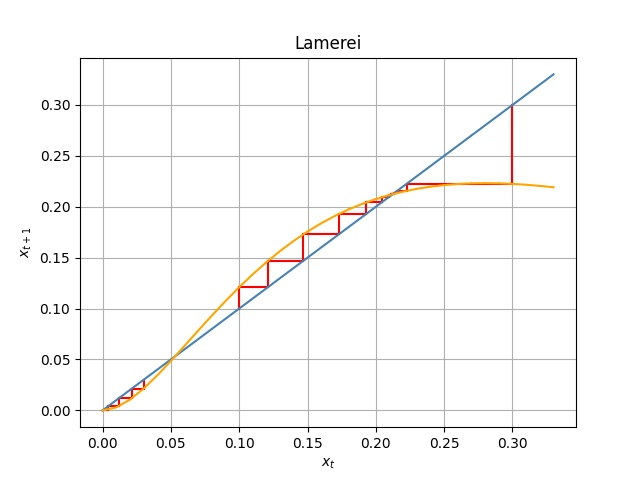
\includegraphics[width=\textwidth]{deterministic/images/lamerei_b_0_56.jpg}

        \captionsetup{justification=centering}
        \caption{Лестница Ламерея модели (\ref{origin}) для \(\beta = 0.56\) и \(x_0 = 0.03\), \(x_0 = 0.1\) и \(x_0 = 0.3\)}
        \label{lamerei_b_0_56}
    \end{figure}

    Давайте зафиксируем начальную численность популяции \(x_0 = 0.03\). На рисунке \ref{lamerei_b_0_56} мы видим, что траектория сходится к нулю. В биологическом смысле это означает, что популяция с течением времени вымирает.

    А теперь зафиксируем начальную численность популяции на уровне \(x_0 = 0.06\). На рисунке \ref{lamerei_b_0_56} видно, что при таких начальных условиях численность популяции сходится к \(x \approx 0.21\).
    
    Очень похожую ситуацию мы можем наблюдать на рисунке \ref{lamerei_b_0_56}. Такой график построен при начальном значении \(x_0 = 0.3\). Значения численности популяции тоже сходятся к устойчивому равновесию. Численность снова стабилизируется.
    
    Теперь рассмотрим ситуацию, когда начальная численность популяции очень большая. Такая ситуация изображена на рисунках \ref{lamerei_x_1_3_b_0_56} и \ref{lamerei2_x_1_3_b_0_56}. Мы видим, что популяция вымирает.

    \begin{figure}
        \centering
        \subfloat[Общий вид лестницы Ламерея]{
            \label{lamerei_x_1_3_b_0_56}
            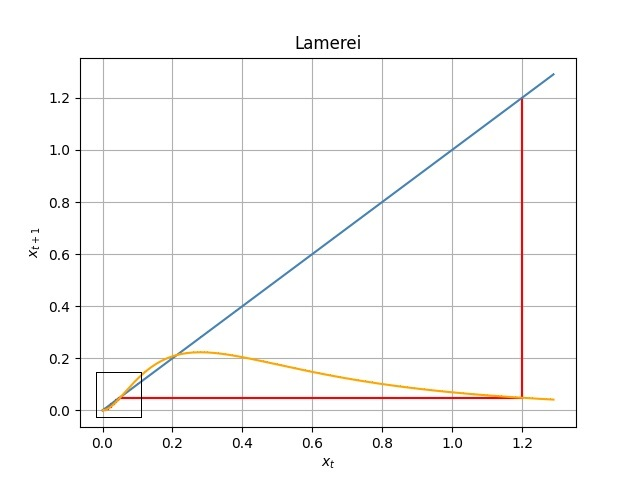
\includegraphics[width=0.9\textwidth]{deterministic/images/lamerei_x_1_3_b_0_56.jpg}
        }

        \subfloat[Дополнение к \ref{lamerei_x_1_3_b_0_56}]{
            \label{lamerei2_x_1_3_b_0_56}
            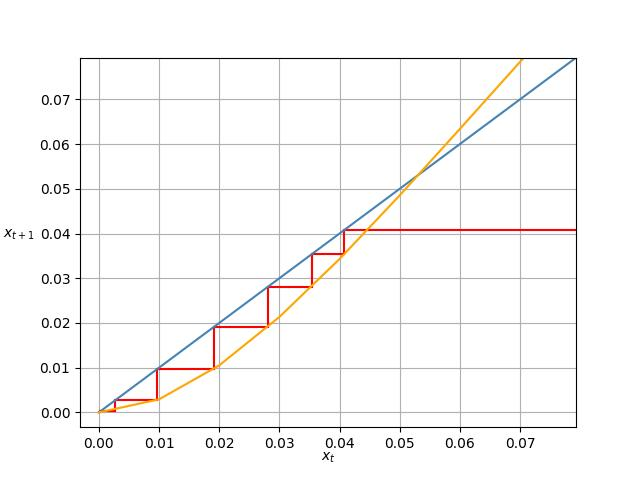
\includegraphics[width=0.9\textwidth]{deterministic/images/lamerei2_x_1_3_b_0_56.jpg}
        }

        \captionsetup{justification=centering}
        \caption{Лестница Ламерея модели (\ref{origin}) для \(\beta = 0.56\) и \(x_0 = 1.3\)}
    \end{figure}

    Таким образом, кроме маленького порогового значения численности популяции существует еще и большое значение, задающие интервал существования популяции. Вне этого интервала популяция вымирает. 
